\chapter{Experimental results}
\label{cpt:experiments}

To evaluate Tribler's current situation and to validate our implementations are working correctly, experiments have been conducted.
In this chapter we elaborate on these experiments and discuss the results. 

\section{Tribler's current state}
To observe if and how the amount of I/O has changed over time, we have performed measurements on four\todo{change if needed} different versions of Tribler using iotop\footnote{\url{http://guichaz.free.fr/iotop/}}.
The hardware used during this experiment can be seen in Table \ref{table:tribler_idle} \todo{Change to VM 15.10 specs}.

\begin{table}[h]
	\centering
	\begin{tabular}{l|l}
		\textbf{Component} 	& \textbf{Specifications} \\ \hline
		Operating System   	& Ubuntu 16.04 LTS \\
		Python version		& 2.7.12 \\
		CPU					& Intel Core i5-2410M \\ 
		HDD					& Samsung 850 EVO 250GB  \\ 
		RAM					& 8 GB DDR3 1600MHz \\
	\end{tabular}
	\caption{Specifications of the setup used during the idle iotop measurement of Tribler 6.6.0-pre-exp.}
	\label{table:tribler_idle}
\end{table}

\begin{figure}[h]
	\makebox[\textwidth][c]{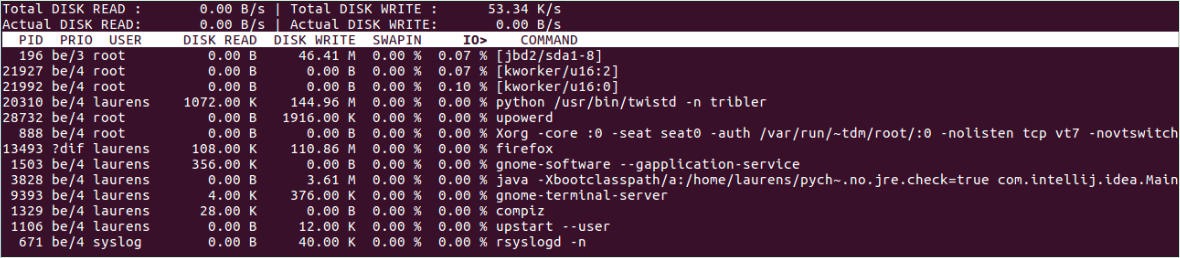
\includegraphics[width=0.95\paperwidth]{experimentation/images/iotop.png}}
	\caption{The output of a two hour idle run.}
	\label{fig:htop_io_idle_run}
\end{figure} 

The results are visible in Figure~\ref{fig:htop_io_idle_run}. \todo{cut unity desktop}
From these results we observe that Tribler I/O has reduced significantly, yet still resides around X\todo{update this}.

\section{I/O breakdown}

\begin{table}[]
	\centering
	\caption{A breakdown of the functions called on StormDBManager.}
	\label{table:breakdown_tribler_idle}
	\begin{tabular}{|l|r|r|l|l|l|}
		\hline
		\textbf{Query}	& \textbf{Amount of calls} & \textbf{Total time (s)} & \textbf{Max}  & \textbf{Average} & \textbf{Min} \\ \hline
		fetchone	& 83036	& 3361.644 	& 0.81436	& 0.04048	& 0.00006 \\ \hline
		fetchall	& 2569	& 22.512	& 0.66344	& 0.00876	& 0.00007 \\ \hline
		execute		& 422	& 2.326  	& 0.20488	& 0.00551	& 0.00007 \\ \hline
		executemany	& 1		& 0.009 	& 0.00915 	& 0.00915	& 0.00915 \\ \hline
	\end{tabular}
\end{table}

To observe the individual components separately, we have created a breakdown of the database queries performed by Tribler and Dispersy.
We have run Tribler idle for one hour and tracked how many times each function in StormDBManager was called by either Dispersy or Tribler and how long it takes between scheduling the query the callback being invoked.
A breakdown of the functions is visible in Table~\ref{table:breakdown_tribler_idle}.
From this table we see that the \enquote{fetchone} function is being called the most, but what does this mean\todo{change and elaborate}

\section{Tribler's responsiveness}

Performance is defined by responsiveness... we measured responsiveness by measuring how many calls were delayed when running idle... next we performed responsiveness measurements using JMeter on the API introduced in Tribler, measuring throughput AND response times, variance etc. in a table. \todo{todo}

\section{Scalability}

If allchannel works, talk about scalability of nodes. \todo{todo}

\section{Validating the performance regression system}

To validate the performance regression system, we have resolved one of Tribler's biggest bottlenecks: Dispersy's blocking database I/O.
To address this problem, we have written Dispersy's I/O to become asynchronous and non-blocking.
To realize this, a new database manager \enquote{StormDBManager} is introduced and 90\%\todo{made up number, need to calculate the actual value.} of Dispersy's functions have been refactored.

